\chapter{Compensazione in frequenza una sonda  e Caratterizzazione di un filtro RC}
\label{chap:Prova2}
\section*{Obbiettivo}
L'obbiettivo della seconda esperienza di laboratorio è stato quello di effettuare la compensazione in frequenza di una sonda e poi di ricavare i diagrammi di Bode di un filtro passabasso passivo RC, i valori di \emph{attenuazione} e \emph{sfasamento} con le relative \emph{incertezze} mediante valutazioni di tipo B.

\section{Compensazione in frequenza di una sonda}
Le sonde costituiscono un componente fondamentale per poter prelevare un
segnale da osservare e da trasferire poi allo strumento.

\begin{figure}[h]
    \centering
    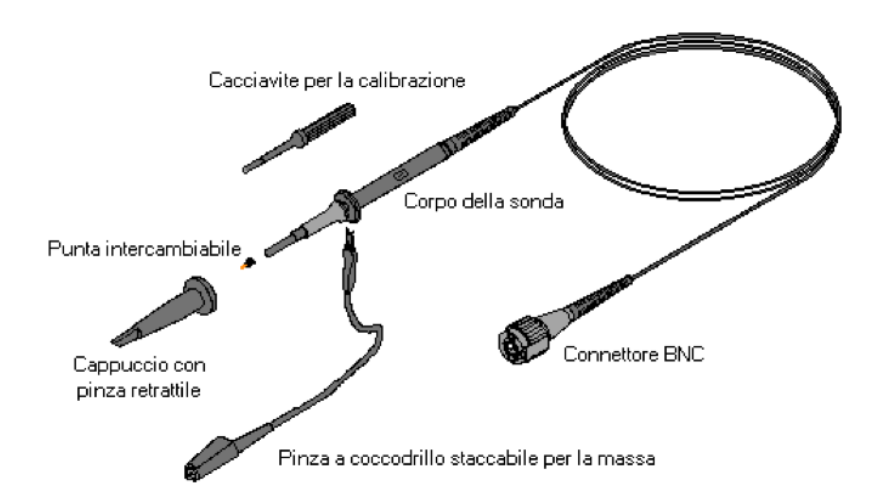
\includegraphics[height=7cm]{sonda.png}
    \caption{Sonda}
    \label{fig:sonda}
\end{figure}

La sonda può essere schematizzata in maniera semplificata come un parallelo di una resistenza e una capacità variabile. L'oscilloscopio d'altra parte ha una certa capacità intrinseca in parallelo ad una resistenza di ingresso. Tale capacità in regime AC può essere un problema, in quanto all'aumentare della frequenza, inizia ad agire come un filtro passa-basso.

Per questo motivo è necessario effettuare la \textbf{compensazione in frequenza della sonda}, cioè impostare il valore della capacità variabile della sonda per andare a compensare gli effeti della capacità di ingresso dell'oscilloscopio, quindi da rendere il sistema sonda+oscilloscopio indipendente dalla frequenza.

\subsection*{}
Per poter effettuare la compensazione, abbiamo collegato il connettore BNC della sonda al canale 1 dell'oscilloscopio. Abbiamo poi sollevato il cappuccio della sonda e l'abbiamo collegata all'occhiello presente nella parte inferiore del dispositivo, che risulta essere la sorgente di onda quadra di ampiezza 5V e frequenza 1.2KHz generata dall'oscilloscopio stesso.

Poichè la sonda fornisce un'attenuazione pari a 10, premendo sul tasto 1 della sezione verticale, è possibile impostare il valore di \emph{Probe} su 10, mediante il tasto presente sotto lo schermo, in modo che la lettura sia riferita all'attenuazione implicita della sonda.

Fatto ciò abbiamo sistemato i valori di $K_v$ e $K_t$ per visualizzare circa 2 periodi e in modo ottimale sullo schermo l'onda quadra.

Abbiamo infine utilizzato un cacciavite vicino al connettore o vicino alla corpo della sonda, per regolare la capacità variabile finchè il segnale visualizzato non è apparso quanto più rettangolare possibile, rispetto alla condizione iniziale in cui erano presenti delle sovra-elongazioni dovute alla sovracompensazione.


\clearpage
\section{Filtro RC} \label{sec:filtroRC}
Il filtro RC è un sistema che effettua sul suo segnale di ingresso una funzione di attenuazione in quanto passivo, cioè composto da componenti passivi quali un condensatore e un resistore in serie.

\begin{figure}[h]
    \centering
    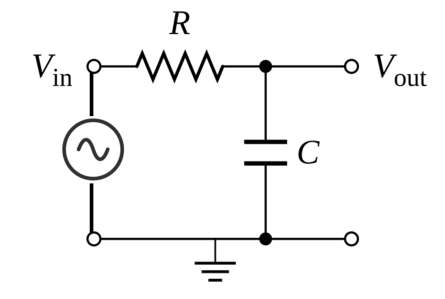
\includegraphics[height=5cm]{filtroRC.png}
    \caption{Filtro RC}
    \label{fig:filtroRC}
\end{figure}
\FloatBarrier

Esso è un filtro passa basso che cioè permette il passaggio delle frequenze al di sotto di una \textbf{frequenza di taglio} e attenua quelle alte. In particolare, l'attenuazione $A$ del filtro RC è definita come:

\[A=\frac{1}{1+j\omega RC}\]

La frequenza di taglio del filtro è definita come la frequenza alla quale la potenza del segnale in uscita dal filtro è pari alla metà della potenza del segnale in ingresso ad esso. Oppure è definita come la frequenza alla quale la tensione disponibile in uscita e $1/\sqrt{2}$ la tensione di ingresso disponibile in banda passante.

La frequenza di taglio teorica si calcola uguagliando il modulo dell'attenuazione $A$ al valore $1/\sqrt{2}$

\[\frac{1}{\sqrt{1+(\omega RC)^2}} = \frac{1}{\sqrt{2}}\]
\[1+(\omega RC)^2 = 2\] 
\[(\omega RC)^2 = 1\]
\[\omega ^2 = \frac{1}{(RC)^2}\]
Ricordando che $\omega = 2\pi f$, si ha che la frequenza di taglio è pari a 
\[f=\frac{1}{2\pi RC}\]

\section{Strumentazione utilizzata}
\subsection*{PCB}
Il PCB (Printed Circuit Board) è una scheda elettronica fornita durante l'esercitazione, sulla quale è stato realizzato un filtro RC, i cui valori di resistenza e capacità sono rispettivamente 10k$\Omega$ e 47nF.

\begin{figure}[h]
    \centering
    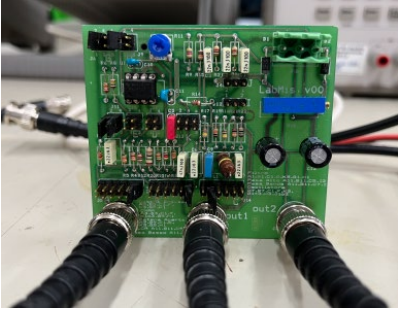
\includegraphics[width=0.9\linewidth, height=6cm]{PCB.png} 
    \caption{PCB}
    \label{fig:pcb}
\end{figure}

\begin{figure}[h]
    \centering
    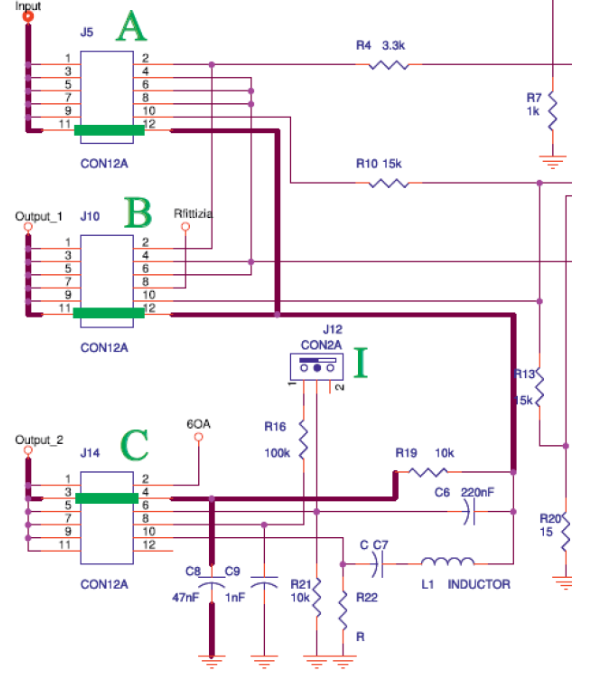
\includegraphics[width=0.9\linewidth, height=14cm]{PCB_RC.png}
    \caption{Configurazione di filtro RC del PCB}
    \label{fig:pcb_rc}
\end{figure}
\FloatBarrier

\clearpage
\subsection*{Oscilloscopio Agilent Hp 54600B}
\begin{figure}[h]
    \centering
    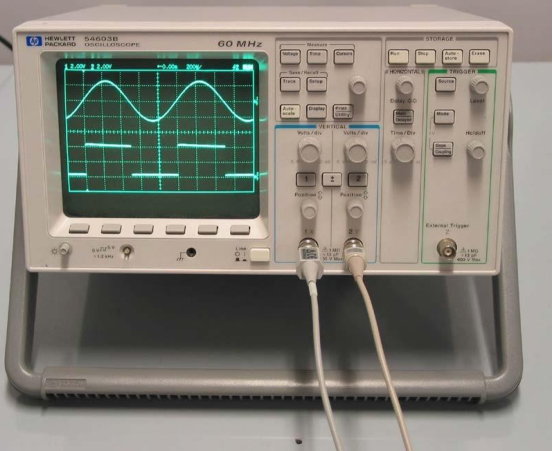
\includegraphics[width=0.9\linewidth, height=9cm]{oscill.png}
    \caption{Oscilloscopio Agilent Hp 54600B}
    \label{fig:oscill}
\end{figure}
\FloatBarrier

\subsection*{Generatore di funzioni Agilent 33120B}
\begin{figure}[h]
    \centering
    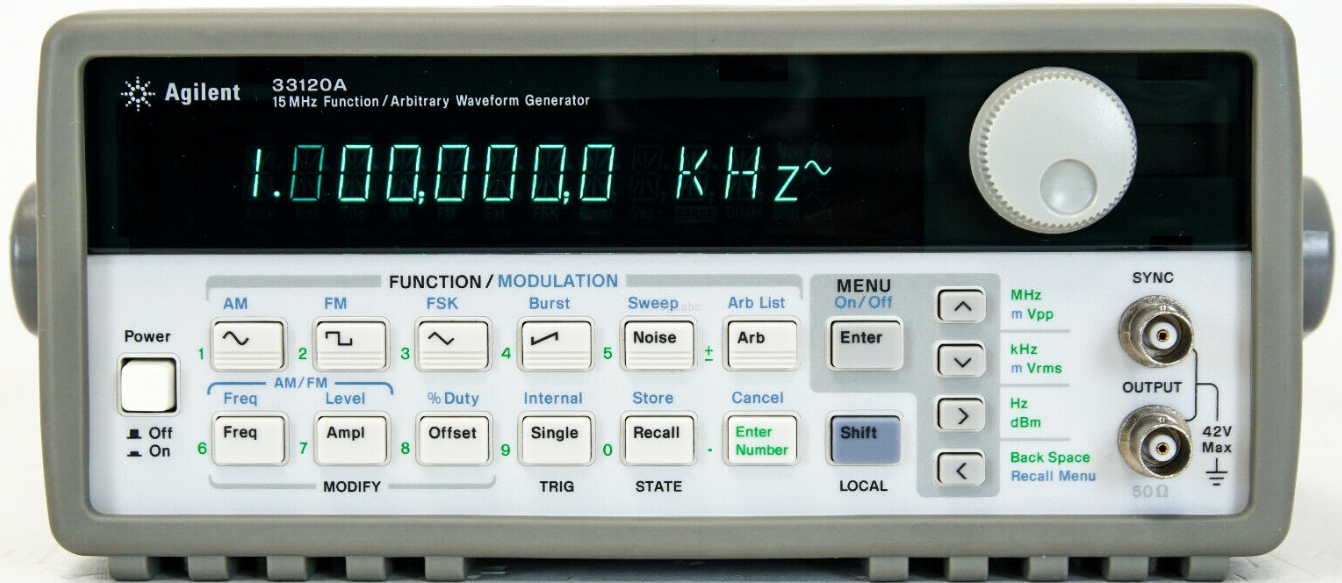
\includegraphics[width=\linewidth, height=6cm]{gen_fun.png}
    \caption{Generatore di funzioni Agilent 33120B}
    \label{fig:gen_fun}
\end{figure}
\FloatBarrier

\subsection*{Cavi di connessione (BNC-BNC)}
\clearpage
\section{Configurazione della strumentazione per la misurazione}
Prima di iniziare ad effettuare le misurazioni del caso, abbiamo configurato tutte le strumentazioni a disposizione. Abbiamo dunque:

\begin{itemize}
    \item Collegato i cavi di connessione secondo la seguente configurazione:
    \begin{itemize}
        \item Uscita del generatore di funzioni all'ingresso (BNC INPUT) del filtro RC
        \item Ingresso del filtro RC (BNC OUTPUT 1) al canale 1 dell'oscilloscopio
        \item Uscita del filtro RC (BNC OUTPUT 2) al canale 2 dell'oscilloscopio
    \end{itemize}
    \begin{figure}[h]
        \centering
        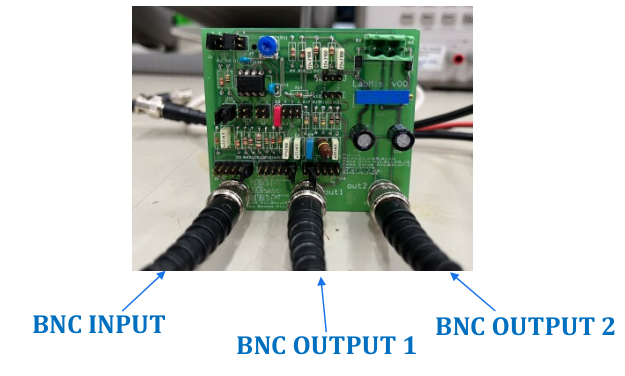
\includegraphics{PCB_bnc.png}
        \caption{Ingressi/Uscite del filtro RC}
        \label{fig:pcb_bnc}
    \end{figure}
    \begin{figure}[h]
        \centering
        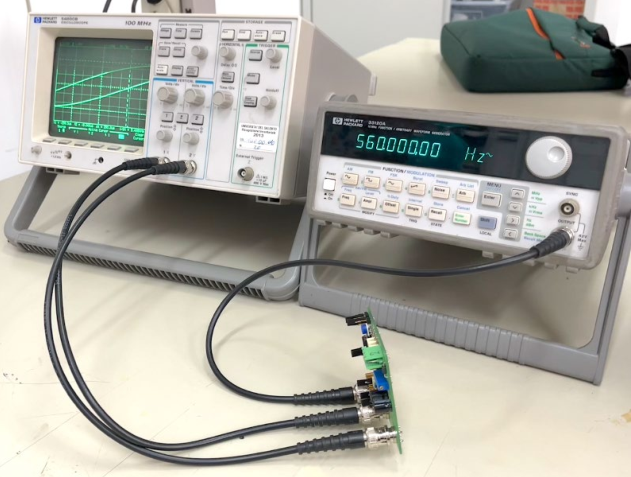
\includegraphics[width=0.9\linewidth, height=6.5cm]{conf_bnc.png}
        \caption{Configurazione dei cavi di connessione}
        \label{fig:conf_bnc}
    \end{figure}
    \FloatBarrier

    \item Avviato il generatore di funzioni impostando una frequenza iniziale di 100kHz mediante il tasto "Freq" e impostato una forma d'onda sinusoidale di ampiezza pari a 5 V.
    
    \'E importante osservare che l'ampiezza visualizzata sull'oscilloscopio è diversa da quella impostata sul generatore di funzioni a causa del disattamento di impedenza tra l'oscilloscpio ed il generatore di funzioni. In particolare, in corrispondenza della tensione picco-picco di 5 V impostata per l'ingresso del filtro, verrà visualizzata una tensione picco-picco di 10 V sul display dell'oscilloscopio.
    \item Avviato l'oscilloscopio su cui visualizzare il segnale d'ingresso del filtro $V_i$ sul canale 1, e il segnale di uscita del filtro $V_o$ sul canale 2.
    Poichè abbiamo utilizzato cavi BNC-BNC e non sonde, abbiamo impostato il valore di \emph{Probe} a 1 mediante l'apposito pulsante posto sotto lo schermo.
    Per migliorare la visualizzazione di entrambi i segnali, abbiamo premuto il pulsante Auto-Scale, che permette all'oscilloscopio di visualizzare entrambi i segnali, uno per ognuno della due metà dello schermo.
    
    Ai fini delle misurazioni da effettuare, abbiamo impostato entrambe le forme d'onda sulla linea di 0 V secondo la seguente procedura per entrambi i canali:
    \begin{enumerate}
        \item Selezione del singolo canale dal rispettivo pulsante della sezione verticale
        \item Impostazione del \emph{Coupling} su Ground mediante il secondo pulsante posizionato sotto lo schermo
        \item Utilizzo della manopola presente sotto la sezione Measure per spostare il riferimento del segnale sulla linea di 0 V
        \item Impostazione del \emph{Coupling} su AC mediante il secondo pulsante posizionato sotto lo schermo  
    \end{enumerate}
\end{itemize}

\clearpage

\section{Misurazioni}

\subsection{Calcolo della frequenza di taglio sperimentale}
Come definito nel paragrafo introduttivo sul filtro RC (\ref{sec:filtroRC}), la frequenza di taglio teorica del filtro RC è pari a
\[f=\frac{1}{2\pi RC}= \frac{1}{2\pi \cdot10^4 \cdot 47 \cdot10^{-9}} = 338,627 Hz\]
Abbiamo dunque ricavato sperimentalmente la frequenza di taglio effettiva. Poichè il segnale in ingresso era pari a 5 V, visualizzati 10V sull'oscilloscopio, allora la frequenza di taglio è quella frequenza in corrisponda della quale l'uscita $V_{o}$ del filtro è pari $10/\sqrt{2} = 7,07 V$.

Abbiamo allora premuto prima sul pulsante \emph{Cursors}, selezionato il cursore $V_1$ posizionandolo per mezzo della mapanopola ad un valore di 3,5 V, 
e il cursore e $V_2$ posizionandolo ad un valore di -3,5 V. In questo modo la distanza tra i due cursori era pari a 7 V.

Andando quindi ad operare sul genereatore di funzioni, abbiamo modificato la frequenza del segnale in ingresso al filtro finché il segnale di uscita (canale 2) non appariva esattamente tangente ai due cursori precedentemente posizionati.
La frequenza per cui tale condizione è stata soddisfatta corrisponde alla frequenza di taglio reale del filtro che è pari a 
\[f_{sperimentale} = 338,63Hz\]

In base al datasheet del generatore di funzioni, il valore dell'incertezza relativa di caso peggiore per misure di frequenza è di 20 ppm (parti per milione), cioè 
\[U_{r,f} = 20 ppm\]
Mentre l'incertezza di caso peggiore è
\[U_f = 338 Hz\cdot U_{r,f} = 338,63Hz \cdot 20 \cdot 10^{-6} = 6,773\cdot10^{-3}\]


\subsection{Misure di tensione picco-picco e $\Delta t$}
Per riuscire a ricavare i diagrammi di Bode dell'attenuazione A del filtro RC, è stato necessario ripetere la stessa procedura di misura, lasciando invariate le condizioni operative, per un totale di 17 diversi valori di frequenza.

Per ogni misurazione abbiamo quindi eseguito i seguenti passi:
\begin{enumerate}
    \item Impostato il valore della frequenza del segnale di ingresso del filtro  sul generatore di funzioni, premendo prima il pulsante \emph{Freq} e poi impostando la frequenza desisderata.
    \item Regolato i valori di $K_{V_i}$ e $K_{V_o}$ mediante le manopole poste nella parte superiore della sezione verticale, in modo da coprire quanto più possibile lo schermo senza tagliare la forma d'onda. In questo modo le misure eseguite sono più accurate e viene ridotta l'incertezza di misura.
    \item Regolato il valore di $K_t$ mediante l'apposita manopola posta nella sezione orizzontale per migliorare la visualizzazione dei segnali.
    \item Premuto il pulsante \emph{Voltage}, situato nella sezione \emph{Measure} e selezionato per ognuno dei due segnali il tipo di misura, cioè tensione picco-picco $V_{p-p}$, mediante gli appositi pulsanti posizionati sotto lo schermo.
    In questo modo i valori di tensione picco-picco di entrambi i segnali vengono automaticamente calcolati dall'oscilloscpio e visualizzati nella parte inferiore dello schermo.
    \item Premuto il pulsante \emph{Cursors} e selezionato i cursori verticali $t_1$ e $t_2$, dagli appositi pulsanti posti sotto lo schermo. Ciascun cursore , mediante la manopola presente sotto la sezione \emph{Measure}, è stato poi collocato in corrispondenza dei punti in cui il corrispondente segnale passava per lo zero. Il valore $\Delta t$ viene calcolato dall'oscilloscopio e visualizzato nella parte inferiore dello schermo. 
    
\end{enumerate}

\clearpage
